\section{Tekniskt bidrag}% "Contributions" -- Syfte.
I denna rapport redogörs för utvecklingen av ett system innehållande en robothand med tre fingrar som fjärrstyrs från en styrhandske. Robothanden designas liknande en mänsklig hand i sina rörelser för att möjliggöra att styrningen blir intuitiv. För att fingrarna ska röra sig flexibelt krävs det att den mekaniska konstruktionen tillåter en rörelse med flera frihetsgrader. För att uppnå detta är handens fingrar konstruerade att aktueras både via genomlöpande senor och stag. Vidare krävs stabila styrsignaler från styrhandsken till robothanden som utnyttjas för att åstadkomma god åtföljning. Detta uppnås genom designade butterworthfilter och programmering där ändrad fingervinkel hos användaren omvandlas till en motsvarande servovinkel. För att användare med olika handstorlek ska uppnå samma resultat är det nödvändigt att kalibrera handsken för varje ny användare. Kalibreringenen sker med hjälp av två knappar som sitter på handskens kretskort.

För att undvika skador på objekt som robothanden hanterar ska ett bibliotek av objekt kunna implementeras i robothandens mikrokontroller som möjliggör objektidentifiering. Varje objekt har ett fördefinierat högsta tryck som robothanden får utsätta den för. Om operatören försöker greppa hårdare än det fördefinierade trycket reglerar robothanden detta för att undvika skada. Objektidentifieringen är baserad på igenkänning av objektets storlek genom att, utifrån vinklar på de styrande servomotorerna, beräkna avståndet mellan de tryckbelastade punkterna på robotfingrarna.

Robothanden följer användarens fingerrörelser tills dess att den greppar ett av flera fördefinerade, kända objekt, då den istället verkar för att hålla objektet med en önskad kraft, tills dess att användaren visar att den vill släppa objektet igen genom att öppna sin hand. Nedan visas ett flödesschema för överskådligt beskriva hur robothanden principiellt fungerar.

\begin{figure}[H]
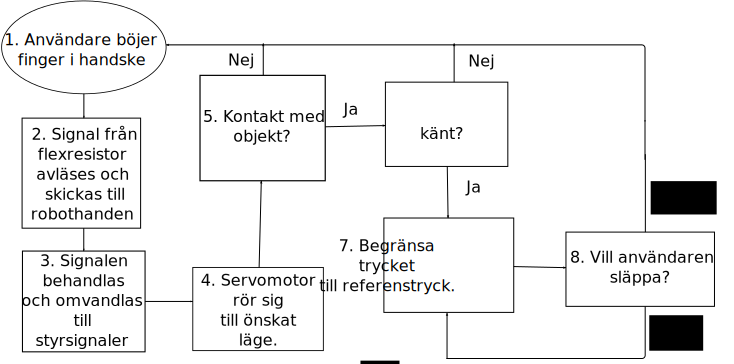
\includegraphics[width=.90\textwidth]{img/flodesschema}
\caption{Flödesschema över en tänkt signals väg genom robothanden.
\comment{det borde inte stå ändringen etc. det är inget som registrerar ``ändringar'' per se, signalen bearbetas kontinuerligt med eller utan ändringar}}
\label{flodesschema}
\end{figure}

\begin{enumerate}
\item Önskat fingerläge ges genom att användaren böjer sitt finger i kontrollhandsken.
\item Flexresistor på kontrollhandsken ändrar resistans.
\item Den ändrade resistansen avläses av en Arduino Micro enhet på kontrollhandsken som skickar den via bluetooth till en Arduino Mega enhet på robothanden.
\item Värdet på resistansen omvandlas till PWM-signal som kalibrerats av användaren vid uppstart.
\item PWM-signaler matas till aktuatorer som ställer sig i önskad vinkel.
\item Feedback från trycksensorer avläses och leder till ett stopp av aktueringen om avläst tryck är högre än fördefinerad gräns.
\end{enumerate}
Robothanden kan delas in i tre delsystem som samverkar för att uppfylla handens funktion. Delsystemen är styrhandske, styrsystem och robothand. Användaren har på sig styrhandsken och styrsystemet verkar för att robothanden ska imitera användarens fingerrörelser tills dess att robothanden kommer i kontakt med ett objekt.



%Detta är just nu en förklaring på vårt systems funktion bara. Bör ingå mer tekniskt? Vilka medel vi använt o så.